\documentclass[11pt,a4paper]{article}
\usepackage[utf8]{inputenc}
\usepackage[T1]{fontenc}
\usepackage{times}
\usepackage[margin=2.4cm]{geometry}
\usepackage{amsmath,amssymb}
\usepackage{booktabs}
\usepackage{array}
\usepackage{longtable}
\usepackage{tikz}
\usetikzlibrary{arrows.meta,positioning}
\usepackage{enumitem}
\usepackage{xcolor}
\usepackage[colorlinks=true,linkcolor=black,urlcolor=blue!60!black]{hyperref}
\usepackage{caption}
\captionsetup{font=small,labelfont=bf}
\setlength{\parskip}{4pt}
\setlength{\parindent}{0pt}

\newcommand{\AD}{\mathrm{AD}}
\newcommand{\ED}{\mathrm{ED}}
\newcommand{\ADV}{\mathrm{ADV}}
\newcommand{\CAR}{\mathrm{CAR}}
\newcommand{\AR}{\mathrm{AR}}

\title{\textbf{Pre-announced, uninformed, and large:\\ the price of moving the premium pension}\\[6pt]
\large Method, data and timeline --- working document}
\author{Alexander Fox and Ludvig Pauli Uväng\\ \small BE451, Stockholm School of Economics. Tutor: Michael Klug.}
\date{14 October 2026 (evening)}

\begin{document}
\maketitle

\begin{center}
\small\itshape Planning document, not thesis text. No result has been computed. Every number below is either a count of what is on disk or a value fixed in advance.
\end{center}

\section{The question and the three regimes}

Since 2024 a new agency, Fondtorgsnämnden (FTN), procures the funds allowed on the premium-pension platform. When a fund loses a procurement, Pensionsmyndigheten redeems the savers' money and moves it to a winner. Most savers do nothing, so the move is automatic. The agency often holds 20 to 44 per cent of a losing fund and sells it in one to three tranches of 5 to 11 per cent of fund assets each. The fund must sell its holdings to pay. The thesis asks:

\begin{enumerate}[nosep]
\item Do the prices of the stocks those funds hold fall on the days they are sold, and by how much relative to what a large uninformed order normally costs?
\item Do the prices recover afterwards?
\item Who pays: the savers who are moved out, or the investors who stay in the losing fund?
\end{enumerate}

The anchor paper is Greenwood and Sammon (2025, \emph{Journal of Finance}), ``The Disappearing Index Effect''. They show that a pre-announced, uninformed demand shock (S\&P 500 index changes) moved prices by 5 to 8 per cent in the 1990s and by less than 1 per cent in the 2010s, because the market learned to absorb it. We replicate their design on Swedish index changes (Part 1), then apply the same tools to a new flow the market has not learned yet (Part 2).

\begin{table}[h]
\centering\small
\begin{tabular}{@{}p{2.6cm}p{5.2cm}p{7.4cm}@{}}
\toprule
Period & What the platform was & Role in the thesis \\
\midrule
2000--Oct 2018 & Open platform: any UCITS fund that signed the agreement, no quality screen, 800+ funds & Institutional background only \\
2019 & New law (Nov 2018): formal thresholds, every fund re-applies; about half are deregistered; SEK 84bn net moved, mostly to AP7 Såfa & Comparison episode: same forced flow, no quality selection, no swing pricing possible for Swedish funds \\
2024-- & FTN procures by category; losers are emptied in tranches; 11 rounds to date & Main test \\
\bottomrule
\end{tabular}
\caption{The three regimes. Only the last two produce forced flows that can be measured.}
\end{table}

\section{Timeline}

\begin{center}
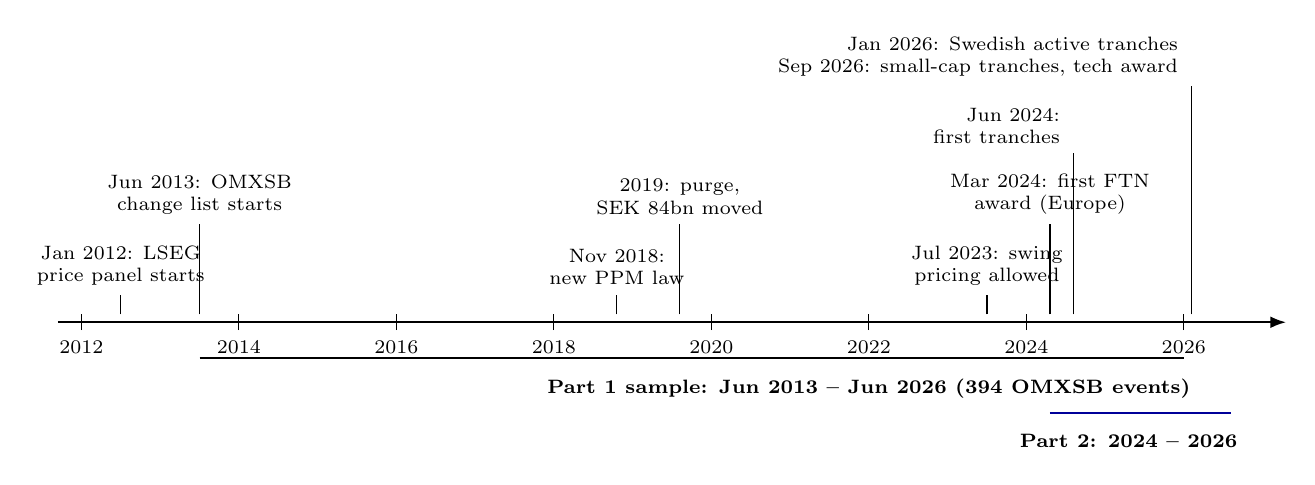
\begin{tikzpicture}[x=1.0cm, every node/.style={font=\scriptsize}]
\draw[-{Latex[length=2mm]}, thick] (-0.3,0) -- (15.3,0);
\foreach \x/\y in {0/2012, 2/2014, 4/2016, 6/2018, 8/2020, 10/2022, 12/2024, 14/2026} {\draw (\x,-0.1) -- (\x,0.1); \node[below] at (\x,-0.12) {\y};}
% level 1
\node[above, align=center] at (0.5,0.35) {Jan 2012: LSEG\\price panel starts};
\node[above, align=center] at (6.8,0.35) {Nov 2018:\\new PPM law};
\node[above, align=center] at (11.5,0.35) {Jul 2023: swing\\pricing allowed};
\draw (0.5,0.1) -- (0.5,0.35); \draw (6.8,0.1) -- (6.8,0.35); \draw (11.5,0.1) -- (11.5,0.35);
% level 2
\node[above, align=center] at (1.5,1.25) {Jun 2013: OMXSB\\change list starts};
\node[above, align=center] at (7.6,1.25) {2019: purge,\\SEK 84bn moved};
\node[above, align=center] at (12.3,1.25) {Mar 2024: first FTN\\award (Europe)};
\draw (1.5,0.1) -- (1.5,1.25); \draw (7.6,0.1) -- (7.6,1.25); \draw (12.3,0.1) -- (12.3,1.25);
% level 3
\node[anchor=south east, align=right] at (12.55,2.15) {Jun 2024:\\first tranches};
\node[anchor=south east, align=right] at (14.05,3.0) {Jan 2026: Swedish active tranches\\Sep 2026: small-cap tranches, tech award};
\draw (12.6,0.1) -- (12.6,2.15); \draw (14.1,0.1) -- (14.1,3.0);
% below
\node[below, align=center] at (10.0,-0.6) {\textbf{Part 1 sample: Jun 2013 -- Jun 2026 (394 OMXSB events)}};
\node[below, align=center] at (13.3,-1.3) {\textbf{Part 2: 2024 -- 2026}};
\draw[thick] (1.5,-0.45) -- (14.0,-0.45);
\draw[thick, blue!60!black] (12.3,-1.15) -- (14.6,-1.15);
\end{tikzpicture}
\end{center}
The remaining dates are deliverables, listed in Section 8.

\section{Part 1: replication of Greenwood and Sammon on OMXSB}

\subsection{Events}
Every addition to and deletion from the OMX Stockholm Benchmark index, June 2013 to June 2026: 394 events (222 additions, 172 deletions) over 27 semi-annual reviews, 325 read from Nasdaq's own releases and 69 from newswire reports. Each event $n$ has a stock $i(n)$, an announcement date $\AD_n$ and an effective date $\ED_n$. Until 2020 the release came at 08:30 before the open, so $\AD_n$ is the release day; from 2021 it came at 18:00, so $\AD_n$ is the next trading day. The lead from announcement to effective date was 14 to 17 trading days until 2020 and 6 trading days from November 2023.

\subsection{Sample filter (their rule)}
\begin{equation}
\mathcal{E}^* = \{\, n : \text{no listing, takeover or delisting of } i(n) \text{ within } [\AD_n - 100,\ \ED_n + 100] \,\}.
\end{equation}
Listing and delisting dates come from the LSEG static table; takeovers are checked by hand for the delisted names.

\subsection{Abnormal returns and windows}
Their measure is market-adjusted, with no factor model:
\begin{equation}
\AR_{it} = R_{it} - R_{m,t}, \qquad R_{m,t} = \text{OMXSPI (price) or OMXSGI (total return)}.
\end{equation}
\begin{align}
\CAR_n^{\text{ann}} &= \sum_{t=\AD_n-1}^{\AD_n+1} \AR_{i(n),t}, &
\CAR_n^{\text{eff}} &= \sum_{t=\ED_n-1}^{\ED_n+1} \AR_{i(n),t}, \\
\CAR_n^{\text{tot}} &= \sum_{t=\AD_n-1}^{\ED_n+1} \AR_{i(n),t}, &
\CAR_n^{\text{rev}} &= \sum_{t=\ED_n+2}^{\ED_n+20} \AR_{i(n),t}.
\end{align}
A four-factor version with Swedish factors is a robustness check, not the main measure, so that the numbers are comparable to theirs.

\subsection{Table 2: means by period}
Separately for additions and deletions, for $p \in \{2013\text{--}17,\ 2018\text{--}20,\ 2021\text{--}23,\ 2024\text{--}26\}$:
\begin{equation}
\CAR_n = \mu_p + \varepsilon_n, \qquad \hat\mu_p = \frac{1}{N_p}\sum_{n\in p}\CAR_n.
\end{equation}
Tests: a joint Wald test that all four $\mu_p$ are equal, the six pairwise differences with Holm correction, and a linear trend in the year. Their decade means are printed beside ours in one sentence.

\textbf{Deviation from the anchor, to be stated.} Their 1,500 events are spread over 40 years. Our 394 fall on 27 review dates, so events on the same date share the market shock. Standard errors are therefore clustered by review date, which they did not need to do. With about 50 events per cell the minimum detectable mean is roughly 2.4 per cent per cell; effects of the size they found in the 1990s would be visible, a 2010s-size effect would not be distinguishable from zero within a cell. The pooled trend and the continuous tracker-demand term below carry the power.

\subsection{Controls (their equation 4) and the tracker-demand extension}
\begin{equation}
\CAR_n^{\text{tot}} = b_1\,\text{turn}_n + b_2\,\text{size}_n + b_3\,\text{vol}_n + \sum_p \gamma_p\,\mathbf 1\{p(n)=p\} + e_n,
\end{equation}
with turn = the stock's turnover in the month before the change minus the value-weighted market turnover, size = market capitalisation on $\AD_n - 1$ over the index's total, vol = the 12-month moving average of the monthly sum of squared daily $\AR$. If $\gamma_p$ falls over time after these controls, the change is in the market, not in the kind of firm being added. Our extension replaces the period dummies with the demand the trackers must execute, in days of normal volume:
\begin{equation}
\CAR_n^{\text{tot}} = b'X_n + \lambda\,\text{Add}_n \times \frac{\text{TrackerAUM}_{t(n)}\, w^{\text{OMXSB}}_{i}}{\ADV_i} + e_n.
\end{equation}

\subsection{Did the trackers trade? (their equation 2)}
From FI's quarterly fund holdings, for the funds that trade in the index's direction at least half the time:
\begin{equation}
\text{NetTrading}_n = 100 \times \frac{\sum_{f\in\text{trackers}}\big(\text{Sh}_{f,i,q+1} - \text{Sh}_{f,i,q-1}\big)}{\text{SharesOut}_{i,q+1}}.
\end{equation}
FI's online archive starts 2018Q4, so this check covers 2019--2026 only.

\subsection{Figures}
Cumulative $\AR$ from $\AD - 100$ to $\AD + 10$ (anticipation), from $\ED - 1$ to $\ED + 100$ (reversal), and the share of volume on $\ED$ within $\pm 22$ days (who supplies liquidity), each by period.

\section{Part 2: FTN forced sales}

The same object as an index change: a large, pre-announced, uninformed flow. Two differences. The treatment is a continuous dose per stock and day rather than in-or-out of an index, and the events are the agency's sale days rather than the index effective date.

\subsection{Event dates}
Per round $r$: the award date $\tau_r$ (FTN press release), the saver letter $\ell_r$ (about two weeks before the first sale), and the tranche days $e$. Tranche days are read from Morningstar's daily fund data as days on which a losing fund $j$ lost at least 5 per cent of its assets:
\begin{equation}
\rho_{jt} = \frac{-\,\text{NetFlow}_{jt}}{\text{TNA}_{j,t-1}}, \qquad e \in \mathcal T_j \iff \rho_{je} \ge 0.05 \text{ and } e \in [\tau_r,\ \tau_r + 60].
\end{equation}
This is already done for about 30 of the 73 losers. The largest Swedish-domiciled losers (Avanza Zero, Storebrand Sverige, LF Sverige Vision, Handelsbanken Sverige, Nordea Swedish Stars, Robur Nordenfond) have only month-end observations in Morningstar; their sale dates are requested from Pensionsmyndigheten.

\subsection{Dose per stock and day}
Expected forced sale in SEK, from the losers' last FI holdings report before the letter ($w_{ij}$ = weight of stock $i$ in fund $j$, $A_j$ = fund assets):
\begin{equation}
S_{ie} = \sum_{j\in\text{losers}} \rho_{je}\, A_j\, w_{ij}, \qquad
B_{ie} = \sum_{k\in\text{winners}} m_{ke}\, w_{ik}, \qquad
F_{ie} = B_{ie} - S_{ie}.
\end{equation}
Here $m_{ke}$ is the money arriving in winner $k$ (from the PPM monthly panel, spread evenly over the month's trading days; a zero-$B$ version is a robustness row). Scaled to days of normal volume:
\begin{equation}
x_{ie} = \frac{F_{ie}}{\ADV_i}, \qquad \ADV_i = \frac{1}{50}\sum_{t=e-60}^{e-11} P_{it}\,\text{Vol}_{it}.
\end{equation}
The formula assumes the fund sells pro rata. FI's post-execution report gives $w^{\text{post}}_{ij}$, so the assumption is checked, and the pre-letter weight is the instrument for the realised sale in a 2SLS robustness row.

\subsection{Predicted impact: the square-root law}
From the market-impact literature (Almgren et al.\ 2005; Tóth et al.\ 2011; Bouchaud et al.\ 2018), the peak impact of a metaorder of $Q$ shares when $V$ trade is $Y\sigma_d\sqrt{Q/V}$ with $Y\in[0.5,1]$. For every stock and tranche day, using no FTN returns:
\begin{equation}
\hat\pi_{ie} = Y\,\sigma_{d,i}\,\sqrt{|x_{ie}|}\;\operatorname{sign}(x_{ie}), \qquad Y = 0.7,\quad \sigma_{d,i} \text{ from } [e-250,\ e-11].
\end{equation}
Everything up to here is computed before any return around an FTN date is opened. It is the part of the pre-analysis plan that is frozen.

\subsection{Abnormal returns and windows}
The same measure as in Part 1, $\AR_{it} = R_{it} - R_{m,t}$, so that the two parts are comparable. Windows: $[-1,+1]$ around each tranche day; $[\text{first}-1,\ \text{last}+1]$ per round; $[\text{last}+2,\ \text{last}+20]$ for reversal; $[-1,+5]$ around the award and the letter.

\subsection{Table 3: the main regression}
Unit: stock $\times$ tranche day, about 2,000 observations.
\begin{equation}
\CAR_{ie}[-1,+1] = \alpha_r + \beta\,\hat\pi_{ie} + \theta' Z_{ie} + \varepsilon_{ie},
\end{equation}
with round fixed effects $\alpha_r$ and $Z$ = log market cap, past 12-month return, Amihud illiquidity, book-to-market, industry.
\begin{equation}
H_0^{(1)}:\ \beta = 0 \ \text{(the market absorbs the flow)}, \qquad H_0^{(2)}:\ \beta = 1 \ \text{(priced like any large order)}.
\end{equation}
Columns: (1) $\hat\pi_{ie}$; (2) the raw dose $x_{ie}$; (3) the sell side only, $-S_{ie}/\ADV_i$; (4) the round window on the cumulative dose. The Swedish index round, with a dose of about 0.02 per cent of market cap per tranche, is reported in its own row as a low-dose treated group and is expected to give $\beta$ indistinguishable from zero.

\subsection{Reversal and anticipation}
\begin{equation}
\CAR^{\text{rev}}_{ir} = \alpha_r + \beta^{\text{rev}}\sum_{e\in r}\hat\pi_{ie} + u_{ir}, \qquad \text{pure price pressure: } \beta^{\text{rev}} \approx -\beta.
\end{equation}
The same regression on the award, letter and pre-tranche drift windows separates three readings: predatory trading (drift with the sign of the sale, recovery larger than the tranche-day move), slow-moving capital (little drift, slow recovery), and sunshine trading ($\beta<1$, the pre-announcement lowered the cost). This is Table 4 and is the first candidate to cut if pages run out.

\subsection{Inference}
\begin{enumerate}[nosep]
\item Standard errors clustered by tranche day (all stocks sold on one day share the market shock), with the wild cluster bootstrap because there are only about 25 clusters.
\item The Kolari--Pynnönen adjusted BMP statistic for the mean standardised $\CAR$ on tranche days, and a calendar-time portfolio (long low-dose, short high-dose) with Newey--West errors.
\item Randomisation inference: reassign $\hat\pi_{ie}$ across stocks within the same tranche day 2,000 times and report the share of placebo $|\hat\beta|$ above the estimate.
\end{enumerate}

\subsection{Power, fixed before unblinding}
$\text{MDE}_\beta = 2.8\,\sigma_{\CAR}/(\sigma_{\hat\pi}\sqrt N)$. With $N\approx 2{,}500$, $\sigma_{\CAR}\approx 3$ per cent and $\sigma_{\hat\pi}\approx 0.5$ per cent, $\text{SE}(\hat\beta)\approx 0.12$, so $\beta=1$ against $\beta=0$ is an eight-standard-error distinction if the law holds. Per round: Swedish active is borderline on its own (large caps, dose 0.5 to 2 per cent of ADV); the small-cap round is well powered (dose 10 to 80 per cent of ADV); pooled with round effects is adequate. Every table reports its MDE in the note.

\section{Part 3: who pays (Table 5, optional)}
A fund with assets $A$ that pays a redemption of fraction $r$ at the unswung NAV sells $rA$ at a proportional cost $c$ (impact plus half the spread), and the cost falls on the remaining holders:
\begin{equation}
D_{je} = \frac{c_{je}\,\rho_{je}}{1-\rho_{je}}, \qquad c_{je} = \sum_i w_{ij}\big(|\hat\pi_{ie}| + \tfrac12\,\text{spread}_i\big).
\end{equation}
Under swing pricing with factor $s_j$ the dilution is $(c_{je}-s_j)\rho_{je}/(1-\rho_{je})$. The test, on fund $\times$ tranche day:
\begin{equation}
R^{\text{NAV}}_{je} - R^{\text{bench}}_{je} = a + \delta_0\, D_{je}(1-\text{Swing}_j) + \delta_1\, D_{je}\,\text{Swing}_j + u_{je}, \qquad H_0: \delta_0 = -1,\ \delta_1 = 0.
\end{equation}
The 2019 purge enters here as a pooled sample: Swedish funds could not swing-price before July 2023, so every 2019 exit is a clean no-swing case. For index losers the power is high (tracking error 3 to 5 bp against 20 to 30 bp of cumulated dilution); for active losers it is low and the result is reported beside the index result.

\section{Data: what each variable is, where it comes from, and its status}

\begin{small}
\begin{longtable}{@{}p{3.6cm}p{3.9cm}p{4.0cm}p{3.6cm}@{}}
\toprule
Variable & Used in & Source and file & Status 14 Oct \\
\midrule
\endhead
Daily close, total return, volume, market cap, shares outstanding, turnover; 1,696 stocks; 2012--2026 & $\AR$, $\CAR$, $\ADV$, turn, size, vol, $x_{ie}$, $\sigma_{d,i}$, $Z$ & LSEG via CodeBook; \texttt{td\_daily\_*.csv} & Downloading: 377 of 1,696 done at 21:15, about 7 s per stock, finishes around midnight \\
Index levels (OMXSPI, OMXSGI, OMXSB, OMXSBGI, OMXS30) & $R_{m,t}$, figures & LSEG; \texttt{indices\_daily.csv} & Cell 6, one minute, after the stock pull \\
OMXSB additions and deletions, $\AD_n$, $\ED_n$ & Part 1 events & Nasdaq releases; \texttt{omxsb\_changes\_2013\_2026.csv} & Done: 394 events; all 152 companies mapped to LSEG codes and verified against prices around their events \\
Tranche days $e$, $\rho_{je}$, $A_j$ & Dose, Table 5 & Morningstar daily valuations via SHoF; \texttt{exit\_days\_by\_loser.csv} & Done for about 30 losers through 30 Sep 2026; refresh to 31 Oct in week 5 \\
Sale dates for the largest Swedish losers & Dose, Swedish active and index rounds & Pensionsmyndigheten, request under offentlighetsprincipen & Email to send; answer in 1 to 3 weeks; without it the index round is month-dated and Swedish active loses 3 of 18 funds \\
Fund holdings $w_{ij}$ & Dose, NetTrading, holdings-staleness check & FI quarterly holdings, \texttt{fi\_YYYYqN.zip} & 4 of 12 quarters on disk; 8 downloads from fi.se remain (two minutes each) \\
Winners' inflows $m_{ke}$, fee savings & $B_{ie}$, cost--benefit & PPM monthly panel; \texttt{ppm\_panel\_2018\_2026.csv} & Done \\
Award and letter dates, winners, losers & Rounds, windows & FTN reports; \texttt{bids\_long.csv} & Done, 11 rounds \\
Swing-pricing status and factor & Table 5 & Fund rules and 2025 annual reports; \texttt{swing\_status\_*.csv} & Done: 11 yes, 38 no, 29 unknown (mostly Luxembourg) \\
Fund NAV and benchmark & Table 5 & Morningstar reinvested prices; fund master & Done; opened only after unblinding \\
Swedish factors (robustness) & Four-factor $\AR$ & SHoF Fama--French page, or Johansson--Sabbatucci--Tamoni & To download; not on the critical path \\
\bottomrule
\end{longtable}
\end{small}

\subsection*{How the stock universe was built}
LSEG's search returns every quote line of every instrument, so the universe was built in three steps and then trimmed. (i) Active primary quote lines on Nasdaq Stockholm and First North (674). (ii) Delisted lines, searched year by year so no query hit the 10,000-row cap: 657 shares that retired between 2012 and 2026. (iii) Every ISIN the losing funds held according to FI, resolved to its home-exchange line, active or delisted, which added about 220 Swedish lines (A-shares, depository receipts) and 319 Danish, Finnish and Norwegian shares. Subscription rights, paid subscription shares, options, preference shares and lines retired before 2012 were removed (394 lines). Delisted companies keep their price history under a code ending in a caret and a date, for example \texttt{KLOVa.ST\textasciicircum G21}; 967 of the 1,696 codes are of this kind. Each OMXSB company was matched by ticker, then by a ticker search, then by name, and every match was verified by pulling prices in a 20-day window around the company's own events. Renamed companies were resolved by hand (ÅF Pöyry to AFRY, Cellink to BICO, NENT to Viaplay, D.\ Carnegie to Hembla, Africa Oil to Meren, Nyfosa to Altra). Klövern's 2013 event lives under the A-share line because the B share did not exist until December 2014.

\subsection*{Holdings gap to raise with Klug}
Only Swedish-domiciled funds report holdings to FI. Of the 73 losers, 35 do. In the Swedish rounds the losers without FI holdings are C WorldWide Sweden, Danske Invest SICAV Sverige, Odin Sverige, Evli Sweden Equity Index, C WorldWide Sweden Small Cap, Evli Swedish Small Cap and, oddly, Indecap Guide Sverige (a Swedish fund; probably an ISIN mismatch, to be checked). For these the weights must come from the funds' own semi-annual reports or from Morningstar's holdings data via SHoF. Until then they are excluded from the dose, which biases $S_{ie}$ down, not up.

\section{What the thesis can conclude}

The design does not test whether a sponsor picks better funds. That was the question of the earlier SSZ-based plan, and it needs years of post-award returns that do not exist yet. What this design can conclude is more concrete, and each conclusion maps to one table.

\begin{enumerate}[nosep]
\item \textbf{A price in SEK for the reform's transitions} (Table 3 and the cost--benefit paragraph). The forced sales in a round move about SEK 10 to 90bn. If $\hat\beta\hat\pi$ averages 0.3 per cent on the sold amount, the Swedish active round alone cost the moved savers about SEK 280m, against the round's fee saving of SEK 79m a year. The thesis can state in one sentence how many years of fee savings each round's transition consumed, with a confidence band. Nobody has produced that number, and it is the number the policy debate needs.
\item \textbf{Who paid, and a fix} (Table 5). If the stayers paid (dilution of the losing funds' remaining holders, who are mostly ordinary retail investors outside the pension system), FTN's decisions imposed a cost on people who had no part in the reform, and swing pricing or a slower execution schedule removes it. That is a recommendation Pensionsmyndigheten can act on, and the thesis can show from the 2019 purge (no swing pricing possible) and the 2024--26 rounds (mixed) whether it works.
\item \textbf{How the state should sell} (Table 4, if kept). The three theories predict different patterns around the award, the letter and the tranche days. Predation says announce less; sunshine trading says announce more; slow-moving capital says spread the sales over more days. The agency already believes the last one (it staggers large funds ``so that sales do not move market prices''). The thesis tests whether that belief is right.
\item \textbf{Why the index effect disappeared} (Table 2 against Table 3). Greenwood and Sammon could not separate two explanations: the market became more liquid in general, or arbitrageurs learned this one flow. The FTN flow is a new, equally pre-announced, equally uninformed flow in the same market, in the same years, with a dose that reaches tens of per cent of daily volume. If the index effect is gone (Table 2) but the FTN effect is present (Table 3), general liquidity cannot be the whole story; the market learns flows one at a time. That is a contribution to their paper's open question, and it is the sentence to put in the abstract.
\end{enumerate}

\textbf{On the sponsor-quality question.} It stays out of the hypotheses, but it does not have to stay out of the thesis. The bid file already holds each bidder's fee, size and past returns at the award date, so Table 1 can describe what FTN chose: the fee cut per round, the share of winners that were already on the platform, and winners' versus losers' trailing returns. Labelled as descriptive, it gives the reader the sponsor's selection rule without claiming a causal effect, and it sets up the question the data cannot yet answer: whether the funds it chose go on to earn the transition cost back.

\section{Is this a good design? An honest assessment}

\textbf{What is strong.}
\begin{itemize}[nosep]
\item The object is new and the data exist. Nothing has been published on FTN's executions, and the dose per stock is built from administrative facts (prior holdings times the agency's stake) that have nothing to do with the stocks.
\item The anchor fits. Greenwood and Sammon ask why a learned flow stopped moving prices; FTN is the same flow before it is learned. The replication and the extension use the same return measure and the same windows, so the two parts speak to each other in one table.
\item There is a parameter with an external benchmark. $\beta = 1$ against the square-root law is a sharper statement than ``the coefficient is significant''.
\item The power is written down before the data are opened, which none of the prize-winning theses did.
\end{itemize}

\textbf{What is weak, and what to do about it.}
\begin{itemize}[nosep]
\item \emph{Large-cap power.} In the Swedish active round the dose is 0.5 to 2 per cent of daily volume for large caps, so a per-day effect of 0.1 to 0.2 per cent is undetectable. The round window and the small-cap round carry the result. If the small-cap tranches slip to November, the thesis is written on Swedish active, Nordic active and the 2024 European round, with small cap added in the last week.
\item \emph{Missing holdings} for the nine foreign-domiciled losers above. Fixable with semi-annual reports; otherwise state the downward bias.
\item \emph{The global active round is frozen} by the Indecap appeal (Förvaltningsrätten i Stockholm, case 4909-26). Its award exists, its execution does not, so it contributes to nothing that measures flows after award. Say so in one sentence.
\item \emph{The square-root law may not hold} for a fund that must deliver cash on a known day. Then $\beta \ne 1$ is the finding, not a failure, provided the MDE is stated.
\item \emph{Part 1 is shorter than theirs} (13 years, 394 events, 27 dates). It is a calibration, not the headline, and the clustering and the MDE say what it can and cannot show.
\item \emph{Pages.} Forty pages including tables. Tables 2, 3 and 5 are the core; Table 4 (anticipation) and the cost--benefit table are the first to cut.
\end{itemize}

\textbf{Decisions for Friday 17 October with Klug.}
\begin{enumerate}[nosep]
\item Sign-off on the specifications above and on the deviation from the synopsis (written).
\item Replication on OMXSB alone, or OMXSB plus OMXS30 (48 events 2005--2026; adds a 2005--2011 pull of three hours and about 20 hand-resolved delisted names).
\item Whether the 2019 purge enters Table 5 as a pooled sample or an appendix.
\item Market-adjusted returns as the main measure (as in the anchor) with the four-factor model as robustness, or the reverse.
\item Whether the cost--benefit is a table or a paragraph.
\end{enumerate}

\section{Work plan}

\begin{table}[h]
\centering\small
\begin{tabular}{@{}p{3.2cm}p{11.8cm}@{}}
\toprule
When & What \\
\midrule
Tonight & Stock pull finishes; index pull (cell 6). \\
Thu 15 Oct & Combine and verify (cell 7): coverage of all 394 events; download the 8 FI files; send the Pensionsmyndigheten request; replication script runs on OMXSB (first unblinded result, not an FTN result). \\
Fri 17 Oct & Gate meeting with Klug: three checks (panel on disk, event list counted, tranche days visible) and the five decisions above. \\
Week of 20 Oct & Dose, $\hat\pi$, MDE recomputed on actual ADV; Table 2 and figures; FTN specifications frozen and dated. Unblind Table 3. \\
Sun 25 Oct & Data freeze. \\
Week of 27 Oct & Tables 3 to 5, robustness, one script per exhibit, clean-machine run. \\
Mon 2 Nov & Full draft to Klug. \\
Early Nov & Morningstar refresh to 31 Oct for the small-cap tranches; outside read; number audit. \\
Fri 20 Nov & Submission-ready. Hard deadline Mon 7 Dec, 10:00. \\
\bottomrule
\end{tabular}
\end{table}

\end{document}
